\documentclass[nofonts,a4paper,11pt]{article}
\usepackage[margin=2cm]{geometry}

\usepackage{graphicx}
\usepackage[colorlinks=true,linkcolor=black,urlcolor=black]{hyperref}

\usepackage{xeCJK}
\setCJKmainfont[ItalicFont={SimHei}]{SimHei}
\setCJKsansfont{SimHei}
\setCJKmonofont{SimHei}

\renewcommand{\figurename}{图}

\title{\textbf{KENMAWR APARTMENTS PROPOSAL}\\SECOND EDITION}
\author{HMW-Alexander}

\begin{document}

\maketitle

\section{基本信息介绍}
\subsection{地理位置和通勤信息}

\begin{itemize}
	\item 详细地址:401 Shady Avenue, Pittsburgh, PA 15206
	\item 位置信息:参见图\ref{fig:cmu-kenmawr},位于Upper Shadyside,CMU东北约2公里\footnote{本提案的图片全部为高清图片,可放大查看细节。地图照片全部来自于谷歌地图,© 2016 Google Inc, used with permission. Google and the Google logo are registered trademarks of Google Inc.}。
	\begin{figure}[!htb]
	\centering
	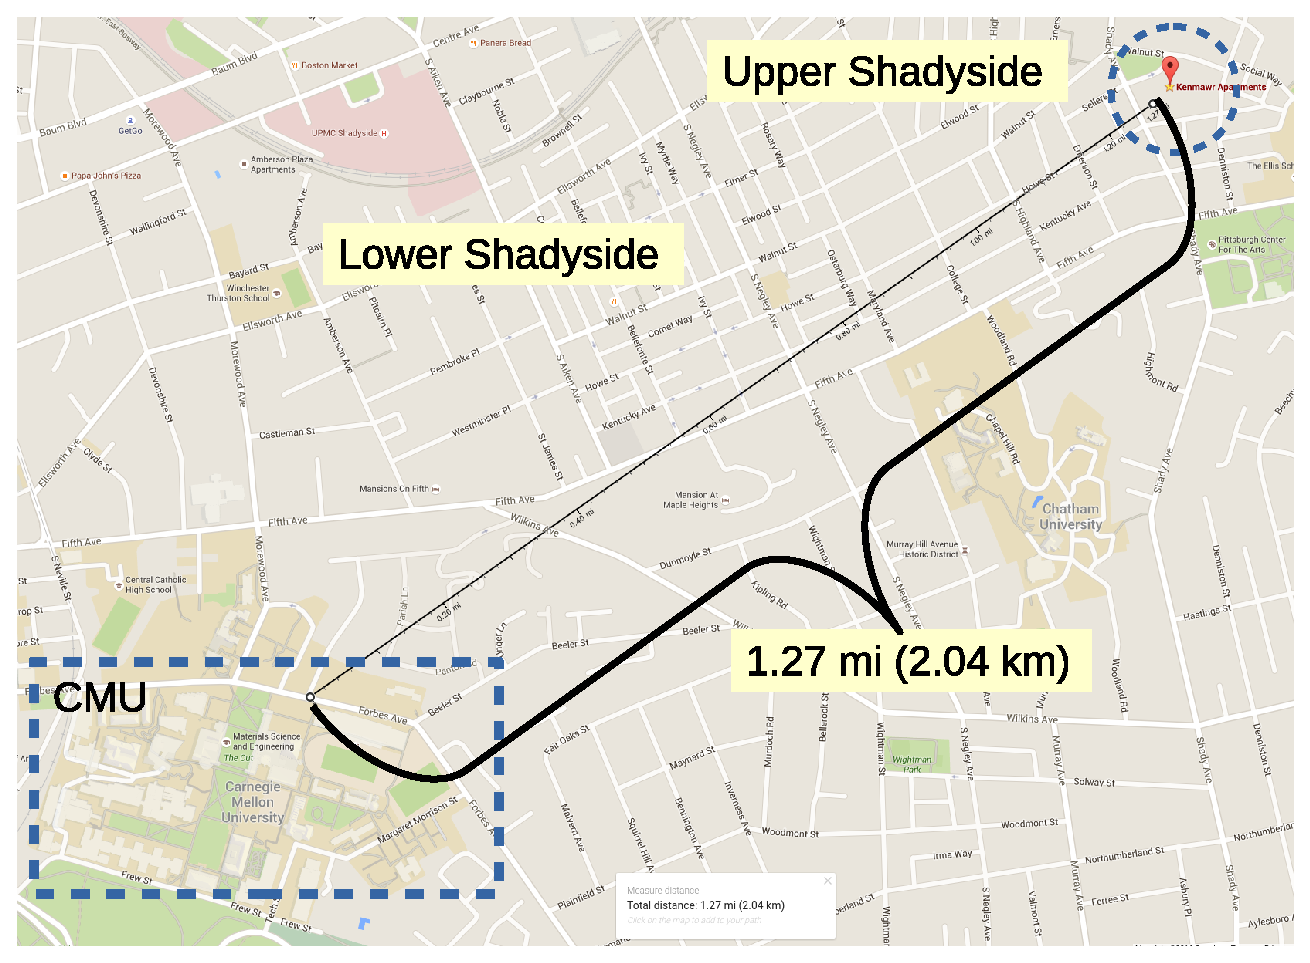
\includegraphics[width=0.6\textwidth]{./img/cmu-kenmawr}
	\caption{Kenmawr Apartments相对于CMU的位置信息}
	\label{fig:cmu-kenmawr}
	\end{figure}
	\item 通勤信息\footnote{推荐大家一个实时公交信息系统:\url{http://www.andysbuses.com/}}:
	\begin{enumerate}
		\item 校车和护送\footnote{\url{https://www.cmu.edu/police/shuttleandescort/index.html}}:
		\begin{itemize}
			\item 公寓楼下就是校车车站 Shady Avenue at Howe Street (图\ref{fig:shuttle}左下)
			\item 上午可以使用B路线校车(图\ref{fig:shuttle}左上)方便到达学校,具体耗时需要实地考察。
			\item 从校车上学方面来讲,Kenmawr相对于Amberson附近的位于Lower Shadyside的公寓有优势。因为Amberson附近校车会沿顺时针走A线路\footnote{\url{https://www.google.com/maps/d/viewer?ll=40.451421\%2C-79.941587\&spn=0.015675\%2C0.027466\&hl=en\&msa=0\&z=15\&source=embed\&ie=UTF8\&mid=zdYfr4QR3ZEM.kLugvZkeznSo}}绕远路,据学长说比走路慢。
			\item 晚上回家会比较远,如果使用AB路线校车(图\ref{fig:shuttle}右上),则需要绕一圈。不过据初步观察,绕道经过的路线有很多餐馆,所以不妨好好享受一下晚餐再回家(校车间隔45分钟)。
			\item 如果晚上回家觉得坐校车不方便,可以考虑6:30 PM之后直接护送到家(图\ref{fig:shuttle}右下蓝色区域)。
			\item 时刻表:
			\begin{itemize}
				\item B线路(工作日):7:15 AM -- 10:45 AM,4:30 PM -- 6:00 PM(每30分钟一班)
				\item AB线路(工作日):11:15 AM -- 3:45 PM,6:30 PM -- 11:00 PM(每45分钟一班)
				\item AB线路(周末):7:15 AM -- 11:45 AM,1:30 PM -- 6:00 PM,7:30 -- 11:15 PM (每45分钟一班)
				\item 护送(每天):6:30 PM -- 6:30 AM (最后接送在6:00 AM)
			\end{itemize}
		\end{itemize}
		\begin{figure}[!htb]
			\centering
			\includegraphics[width=0.8\textwidth]{./img/shuttle}
			\caption{Kenmawr Apartments校车与护送}
			\label{fig:shuttle}
		\end{figure}
		\item 公交:
		\begin{itemize}
			\item 只有两路公交可以使用,分别是71B和71D(图\ref{fig:bus})。
			\item 都需要步行一段距离,全部时间算下来15--18分钟。
			\item 可以考虑用作回家的通勤工具,公交凭学生卡免费。
			\item 从公交方面来讲,Kenmawr没有松鼠山附近公寓的公交多。
			\item 时刻表:\url{http://www.portauthority.org/rt/71d.pdf}。
		\end{itemize}
		\begin{figure}[!htb]
			\centering
			\includegraphics[width=1.0\textwidth]{./img/bus}
			\caption{Kenmawr Apartments公交线路}
			\label{fig:bus}
		\end{figure}
		\item 骑行和开车:
		\begin{itemize}
			\item 骑行需要13分钟(图\ref{fig:bicycle}左)。之所以要绕道,据学长说大道上是没有自行车道的。
			\item 开车需要10分钟左右(图\ref{fig:bicycle}右)。Kenmawr提供200个停车位,每个车位每月100刀。
		\end{itemize}
		\begin{figure}[!htb]
			\centering
			\includegraphics[width=1.0\textwidth]{./img/bicycle}
			\caption{Kenmawr Apartments骑行和开车}
			\label{fig:bicycle}
		\end{figure}
	\end{enumerate}
\end{itemize}

\subsection{周边环境}

\begin{itemize}
	\item 餐厅(图\ref{fig:resteraunt})
	\begin{itemize}
		\item 没有松鼠山的餐厅多,中国餐厅也不多。
		\item 500米范围内有一家中国餐厅China Garden。
		\item 据学长说,S Highland Ave上有很多餐厅(公寓西北500米内),但是没有中餐厅。
		\item 同样据学长说,有几家中国外卖只限中午送。
		\item 所以还是学学做饭吧。
	\end{itemize}
	\begin{figure}[!htb]
		\centering
		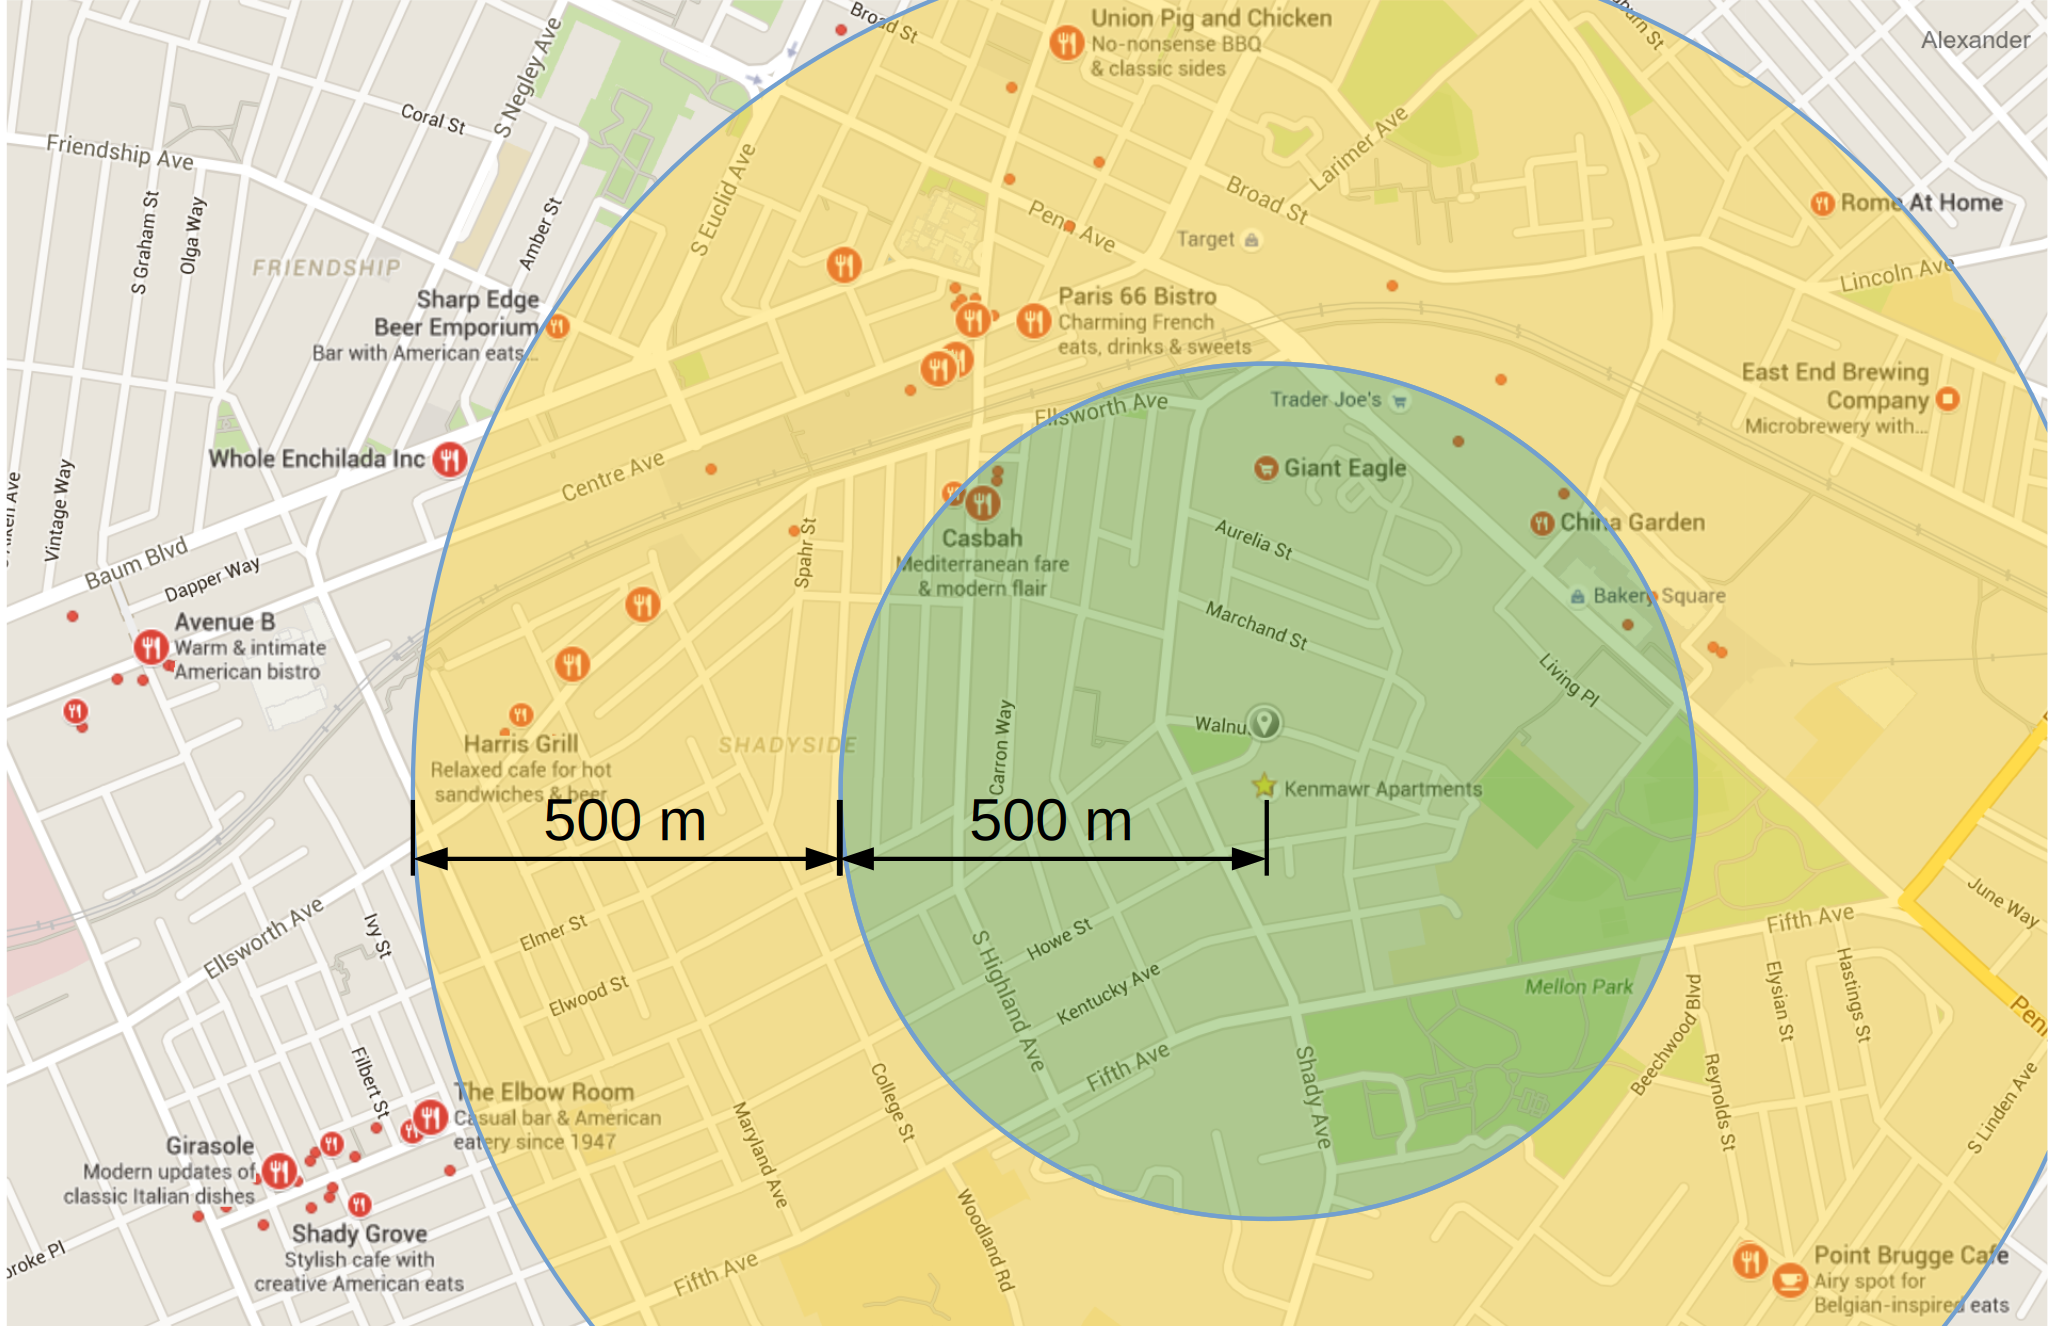
\includegraphics[width=0.6\textwidth]{./img/resteraunt}
		\caption{Kenmawr Apartments周边餐厅情况}
		\label{fig:resteraunt}
	\end{figure}
	\item 超市\footnote{关于超市的所有描述均转自学姐aiweix。}
	\begin{itemize}
		\item Kenmawr附近有Giant Eagle, Trader Joe, CVS 和 Target四大超市,步行5分钟内均可到达。
		\item 另外,周围还有日本超市和Wholefoods, 步行15分钟内可达。
		\item 还有一个对于大家生活品质很重要的地方,就是lotus 中国超市,公寓附近有86和88两路公交直达哦。
		\item 最后,经常去downtown的同学,kenmawr附近还有P1系列公交,可以走公交专线直达downtown, 省时,省力,省心。
	\end{itemize}
	\item 公园
	\begin{itemize}
		\item Mellon Park(图\ref{fig:mellonpark})散心的好去处。
		\begin{figure}[!htb]
			\centering
			\includegraphics[width=0.6\textwidth]{./img/mellonpark}
			\caption{Mellon Park照片选编}
			\label{fig:mellonpark}
		\end{figure}
	\end{itemize}
	\item 不安全区域\footnote{本人无任何种族歧视倾向。}
	\begin{itemize}
		\item 据学长说,CMU周围最不安全的两个区分别是East Liberty(黑人区)和Wilkinsburg(枪击案就在那)。
		\item 其中East Liberty位于Kenmawr北约1公里(图\ref{fig:eastliberty}),所以大家没事不要随便去北边转。
		\begin{figure}[!htb]
			\centering
			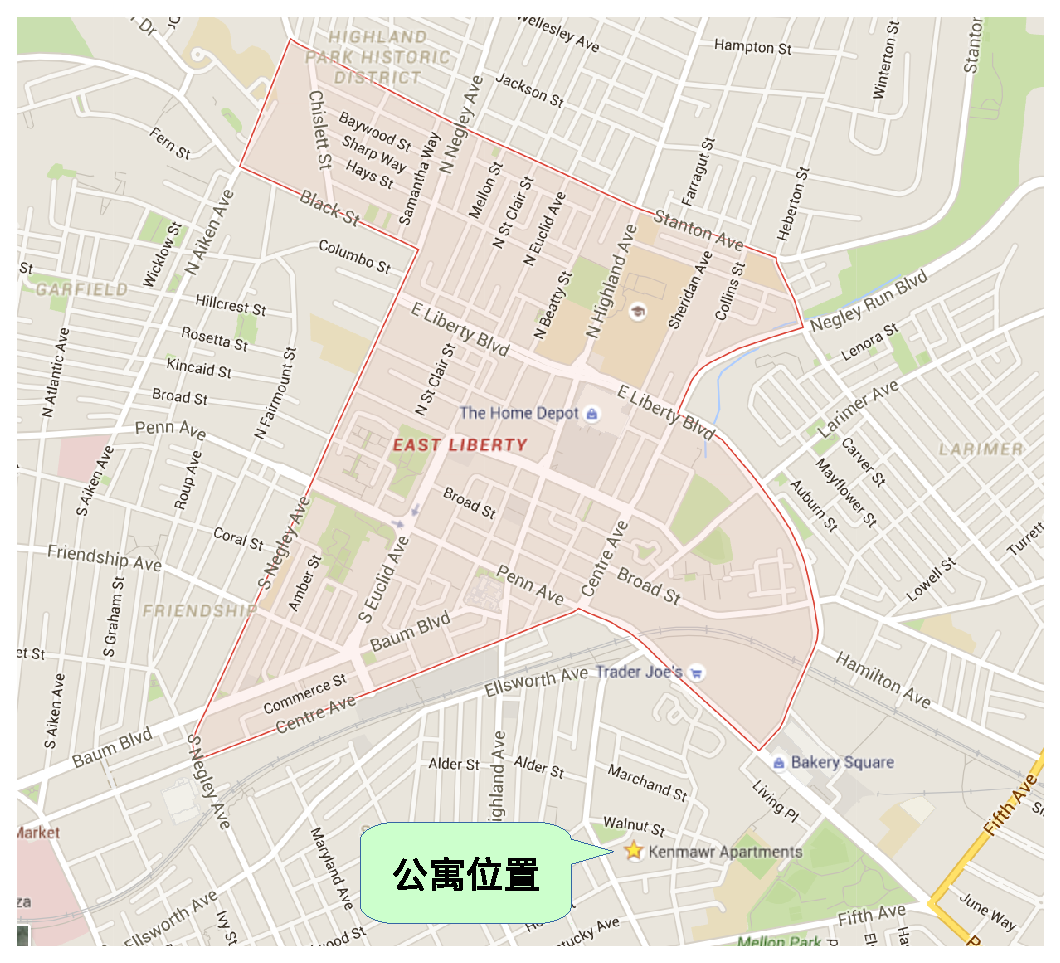
\includegraphics[width=0.6\textwidth]{./img/eastliberty}
			\caption{East Liberty}
			\label{fig:eastliberty}
		\end{figure}
	\end{itemize}
\end{itemize}

\subsection{公寓信息}

\begin{itemize}
	\item 简介\footnote{关于公寓的简介均转自学姐aiweix。}
	\begin{itemize}
		\item Kenmawr(图\ref{fig:apartment})是在CMU附近高端大气上档次的公寓了,楼内有很多中国留学生居住。
		\item 公寓里面有收发室,不用担心包裹丢失的问题。
		\item 而且,公寓还有免费的健身房(图\ref{fig:fitness})可以使用,每天跑跑更健康。
		\item 另外,公寓楼下设停车场,还有类似于超市的shopping cart, 买完东西可以把东西放在shopping cart乘电梯上楼,省力,更省心。
		\item 看门的大叔大爷们都十分nice, 总之就是一个很温馨,安全,舒适的公寓啦!
		\item -------------------以下来自聊天记录,关于暖气-------------------
		\item “我之前住的公寓,冬天会很冷”
		\item “这个公寓的暖气特别好,不会受冻”
		\item “所以我要提醒你,要看暖气好不好”
		\item “夏天看房子根本看不出来,我刚来的时候也完全没想到暖气这回事”
		\item “美国这边很多房子都很旧,设备也很旧”
		\item “我现在住的这个是比较新的了”
		\item -------------------以下来自聊天记录,关于其他住户-------------------
		\item “楼里还有很多日本人住,经常会有日语学习班啥的”
		\item “额,有的,但不多,这边住的日本人大多数是在这边工作的,一家人这样”
		\item “还有一些美国的老头老太太在这边住养老”
		\item -------------------以下来自聊天记录,关于健身房-------------------
		\item “额,我不知道多大算大,这个肯定不小”
		\item “不挤,没有很多人来健身,我每天都会去”
	\end{itemize}
	\begin{figure}[!htb]
		\centering
		\includegraphics[width=0.8\textwidth]{./img/apartment}
		\caption{Kenmawr Apartments外景}
		\label{fig:apartment}
	\end{figure}
	\begin{figure}[!htb]
		\centering
		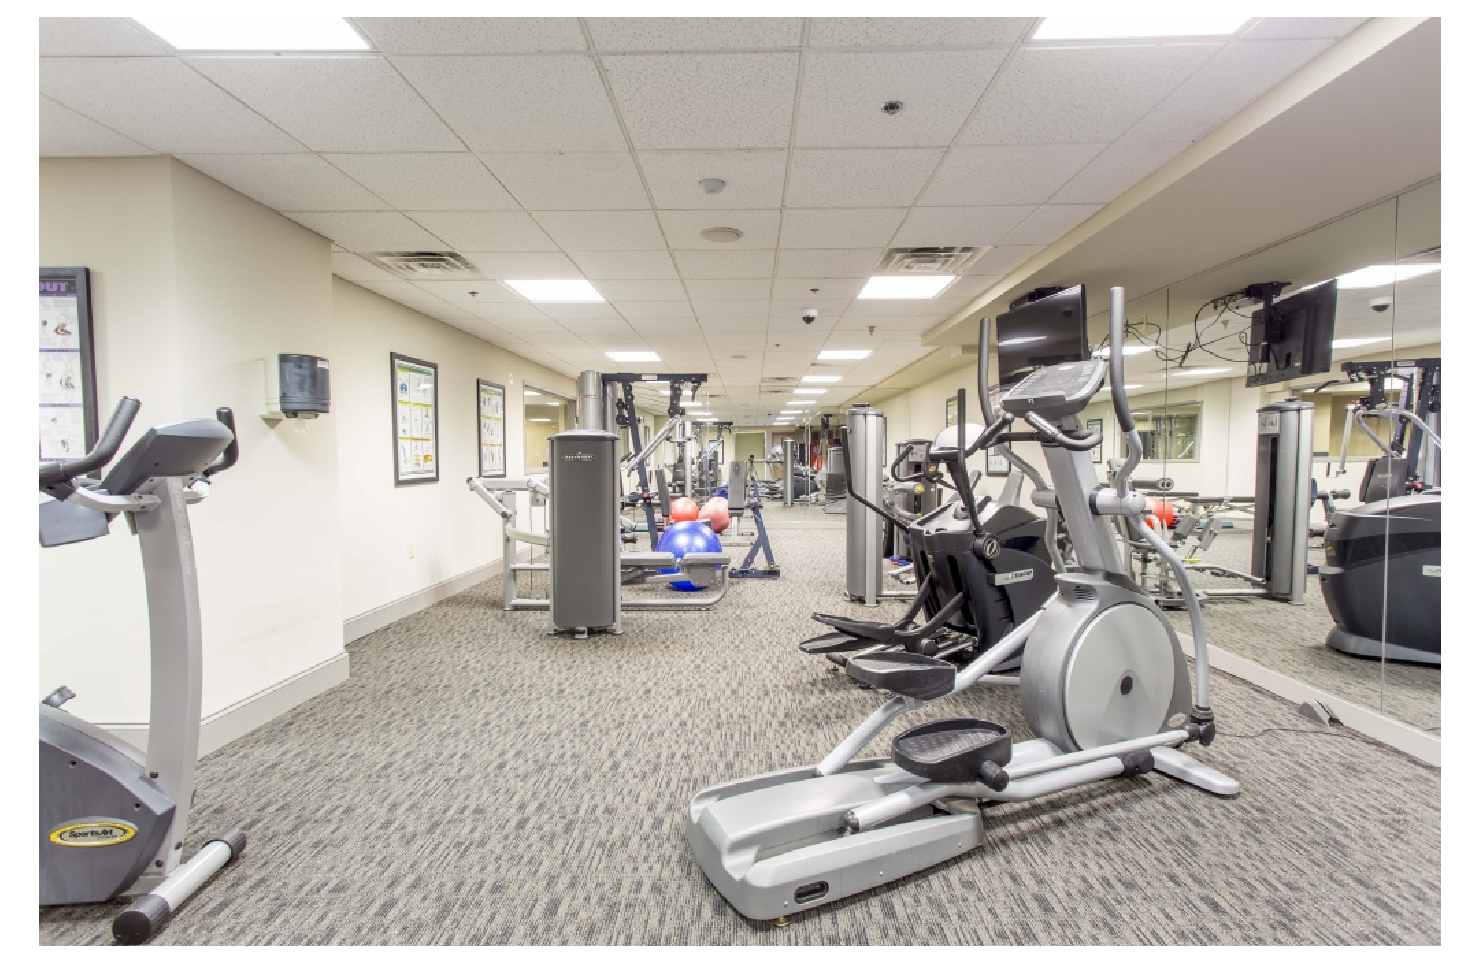
\includegraphics[width=0.8\textwidth]{./img/fitness}
		\caption{Kenmawr Apartments健身房}
		\label{fig:fitness}
	\end{figure}
	\item 户型和费用
	\begin{itemize}
		\item 我比较中意两种户型(图\ref{fig:floorplan})。如果两人合租则选择BR2/BA2,如果三人合租则选择BR3/BA2。
		\item 由于客厅的隐秘性不好,所以不打算出租,而是作为公共休闲区域或是大书房。
		\item 卫生间两个,所以男女生可以一起合租而避免尴尬。
		\item 公寓价格\footnote{http://www.apartments.com/kenmawr-apartments-pittsburgh-pa/n9b9zrp/}
		\begin{itemize}
			\item BR2/BA2为1695刀
			\item BR3/BA2为2050刀
		\end{itemize}
		\item 额外费用\footnote{http://www.apartments.com/kenmawr-apartments-pittsburgh-pa/n9b9zrp/}
		\begin{itemize}
			\item Gas, Water, Heat, Trash Removal: Free
			\item Assigned Garage Parking [Recurring Expenses]: \$100
			\item Security Deposit [One Time Expenses]: \$1,195 -- \$2,050
		\end{itemize}
		\item 所以粗略平均下来每人700--800刀
	\end{itemize}
	\begin{figure}[!htb]
		\centering
		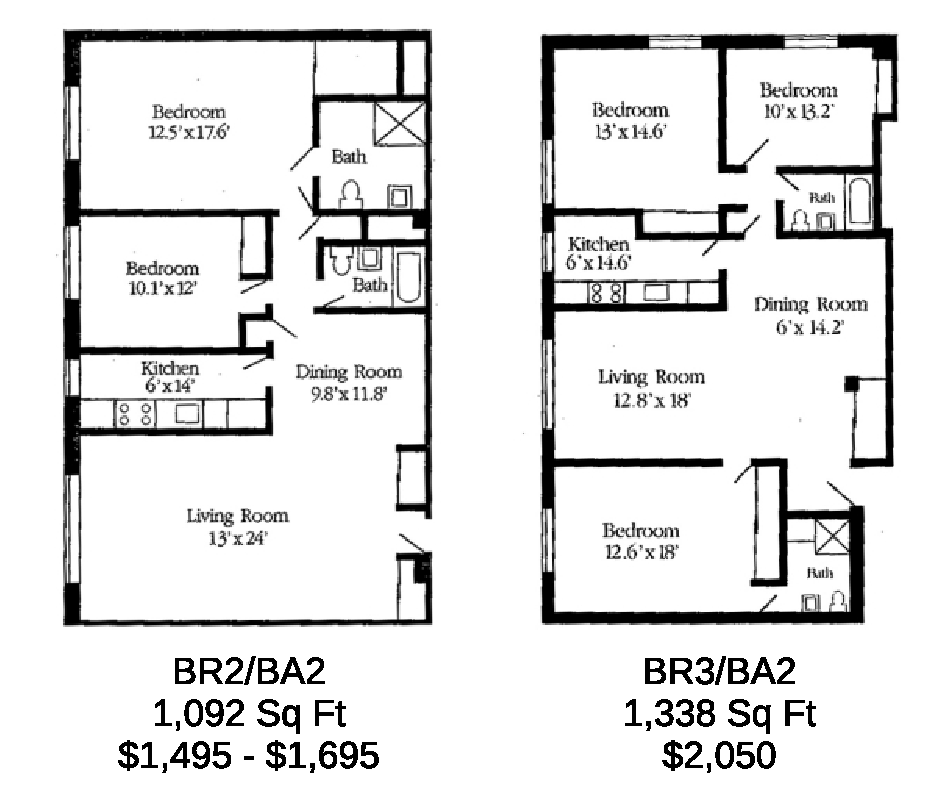
\includegraphics[width=0.8\textwidth]{./img/floorplan}
		\caption{Kenmawr Apartments房型}
		\label{fig:floorplan}
	\end{figure}
\end{itemize}

\section{合租计划}

\subsection{租房时间}
\begin{itemize}
	\item 开始时间:2016年08月01日
	\item 持续时间:本人希望尽量少折腾,最好不要少于2年,最好5年。
	\item 租房决定截止期:还在联系公寓管理人进行确定,有消息会进行更新。
\end{itemize}

\subsection{费用分摊}
\begin{itemize}
	\item 原则上基于使用面积和公私属性,对特殊情况进行协商处理。
	\item 共用面积平摊,包括客厅,餐厅,厨房。
	\item 私用面积自担,包括卧室,卫生间(合用的平摊)。
	\item 电网费用、公用的家居、厨具、餐具、卫生用具平摊。
	\item 私人家居,生活用品自担。
	\item 做饭等提供公共服务的行为,鼓励基于协商的公摊费用调整。
\end{itemize}

\subsection{室友选择}
以下内容同样适用于短期转租的房客,同时短租需通过协商征得其他合租人同意。
\begin{itemize}
	\item 男女不限。
	\item 本人极度不能忍烟味,所以只招不吸烟的室友。
	\item 本人不喝酒,但是室友不做特别限制,最好不要宿醉或狂酒。
	\item 最后就是性格开朗,积极向上,爱干净,无不良嗜好,懂得包容沟通。
\end{itemize}

\subsection{关于顺利租到房子}
\begin{itemize}
	\item 由于好房源抢手,所以需要有意向者尽快联系,并尽快提供所需材料(见“3.公寓管理员信息反馈”)。
	\item 我向学院申请了暑期开始博士项目,同时老板同意并提供资金支持,所以学院会提前处理我的移民材料。我会尽快拿到I-20表和签证,然后5,6月份去CMU。
	\item 所以,如果合租人还没有拿到所需材料,我可以先以个人身份租房,然后等你们来了和公寓签合同加入到我的lease中。(所需材料是一样的)
	\item 最后希望合租人不要放我的鸽子。
\end{itemize}

\section{公寓管理员信息反馈}
刚收到公寓管理员关于房源和预约的回信。信息还会持续更新。
\begin{itemize}
	\item 房源
	\begin{itemize}
		\item 目前有9套房可用:\\
		\begin{tabular}{|c|c|c|c|c|}
			\hline
			D-702 & Two Bedroom One Bath & Model B3 & Standard & \$1395 \\
			B-708 & Three Bedroom Two Bath & Model C & Standard & \$2050 \\
			D-208 & Two Bedroom One Bath & Model B5 & Updated & \$1595 \\
			C-702 & Two Bedroom Two Bath & Model B4 & Updated & \$1695 \\
			D-506 & One Bedroom One Bath & Model A & Standard & \$1295 \\
			D-401 & Two Bedroom Two Bath & Model B4 & Standard & \$1495 \\
			D-806 & One Bedroom One Bath & Model A & Standard & \$1295 \\
			B-702 & Two Bedroom One Bath & Model B3 & Standard & \$1395 \\
			B-407 & Two Bedroom Two Bath & Model B3 & Standard & \$1395 \\
			\hline
		\end{tabular}
		\item 2016年05月15号有3套房可用:\\
		\begin{tabular}{|c|c|c|c|c|}
			\hline
			D-406 & Three Bedroom Two Bath & Model C & Standard & \$2050 \\
			B-706 & One Bedroom One Bath & Model A & Standard & \$1295 \\
			B-806 & One Bedroom One Bath & Model A & Standard & \$1295 \\
			\hline
		\end{tabular}
		\item 2016年06月15号有2套房可用:\\
		\begin{tabular}{|c|c|c|c|c|}
			\hline
			C-705 & One Bedroom One Bath & Model A & Standard & \$1295 \\
			A-305 & Two Bedroom One Bath & Model B & Standard & \$1395 \\
			\hline
		\end{tabular}
		\item 关于8月份的房源,管理员还在等租户的消息,他们要求提前60天告知,所以最迟6月份应该有消息。
	\end{itemize}
	\item 预约
	\begin{itemize}
		\item 可以预约,但是需要的材料估计大家得等到4,5月份才能拿齐。
		\begin{itemize}
			\item 完整填写 "Philadelphia Management and Companies Application Form",不要忘了在底部签名和附上50刀申请费。费用以汇票、现金支票、银行支票、或者个人支票支付。(大家如果一起来合租的话,我们可以委托在匹兹堡的同学或学长先行垫付)
			\item 分开提交保证金,金额相当于一个月房租,形式同上。
			\item 在返回申请表的时候,请附上photo ID的复印件(如驾照,护照和签证,学生卡)。
			\item 请提供任意一种以下材料(自动忽略不相关的):
			\begin{itemize}
				\item 学校的offer letter或acceptance letter
				\item 你的I20/J1/F1/ form (如果是留学生)
			\end{itemize}			
		\end{itemize}
		\item 如果有一同的申请人,以上需全部提供,但是申请费用为25刀。
		\item 以上材料在申请开始后5个工作日内无法提供,则视为失败,预约将取消。(这里我还在向管理员咨询如何保证租到想要的房子[secure a unit now])
	\end{itemize}
\end{itemize}


\end{document}